% !TEX root = mth727_lecture_notes.tex


\chapter[Relative Homotopy Groups]{Relative \\ Homotopy Groups}
\chaptermark{Relative Homotopy Groups}
\label{RELATIVE HOMOTOPY GPS CHAPTER}
\thispagestyle{firststyle}

\begin{notation}
Let $X \subseteq A_{1} \subseteq A_{2}$ and $Y \subseteq B_{1}\subseteq B_{2}$. 
By a map $f\colon (X, A_{1}, A_{2}) \to (Y, B_{1}, B_{2})$ we will understand 
a map $f\colon X\to Y$ such that $f(A_{i})\subseteq B_{i}$ for $i=1, 2$. 
A homotopy of such maps is a homotopy $h\colon X\times [0, 1] \to Y$ such that 
$h_{t}(A_{i})\subseteq B_{i}$ for $i=1, 2$ and all $t\in [0, 1]$. 
\end{notation}


\begin{notation}
For $n\geq 1$ let $J^{n-1}$ denote the subspace of $I^{n} = I^{n-1}\times I$ given by 
\[
J^{n-1} = I^{n-1}\times \{1\} \cup \pint^{n-1}\times I
\]
We have: $I^{n} \subseteq \pint^{n} \subseteq J^{n-1}$.
\begin{equation*}
\begin{tikzpicture}[scale=1.7]
\filldraw[line width=2pt, fill=mygray1] (0, 0) rectangle (1, 1) node[pos=0.5] {$I^{n}$};
\draw[red, line width=2pt, cap=rect] (0, 0) -- (0, 1) -- node[above] {$J^{n-1}$}
(1, 1) -- (1, 0);
\fill[red] (0, 0) circle (0.05);
\fill[red] (1, 0) circle (0.05);
\end{tikzpicture}
\end{equation*}


\end{notation}


\begin{definition/proposition}
\label{HIGHER REL HOMOT GPS DEF}
Let $x_{0}\in A \subseteq X$. For $n\geq 2$, the \emph{$n$-th relative homotopy 
group} of $(X, A, x_{0})$ is the group $\pi_{n}(X, A, x_{0})$ whose elements 
are homotopy classes of maps $\omega\colon (I^{n}, \pint^{n}, J^{n-1}) \to (X, A, x_{0})$. 

\begin{equation*}
\begin{tikzpicture}[scale=1.7]

\filldraw[line width=2pt, fill=mygray1] (0, 0) rectangle (1, 1) node[pos=0.5] {$X$};
\draw[red, line width=2pt, cap=rect] 
(0, 0) -- node[left] {$x_{0}$}
(0, 1) -- node[above] {$x_{0}$}
(1, 1) -- node[right] {$x_{0}$} (1, 0);
\fill[red] (0, 0) circle (0.05);
\fill[red] (1, 0) circle (0.05);
\node[below] at (0.5, 0) {$A$};
\draw[thick, ->, >=latex] (1.5, 0.5) -- node[anchor=south] {\small $\omega$} (2.0,0.5);
\node at (2.5, 0.5) {$X$};
\end{tikzpicture}
\end{equation*}

Multiplication in  $\pi_{n}(X, A, x_{0})$ is defined as follows. 
If $\omega, \tau\colon (I^{n}, \pint^{n}) \to (X, x_{0})$ then 
\[[\omega]\cdot [\tau] = [\omega\ast\tau]\]
where $\omega\ast\tau\colon (I^{n}, \pint^{n}) \to (X, x_{0})$ is given by 
\[
(\omega\ast \tau)(s_{1}, s_{2}, \dots, s_{n}) = 
\begin{cases}
\omega(2s_{1}, s_{2}, \dots, s_{n}) & \text{ for } s_{1}\in [0, \frac{1}{2}] \\
\tau(2s_{1} -1, s_{2}, \dots, s_{n}) & \text{ for } s_{1}\in [\frac{1}{2}, 1] \\
\end{cases}
\]

\begin{equation*}
\begin{tikzpicture}[scale=0.9]
\draw[line width=1.6pt, fill=mygray1] (0,0) rectangle  node[anchor=center] {$\omega$} (1,2);
\draw[line width=1.6pt, fill=mygray1] (1,0) rectangle node[anchor=center] {$\tau$}(2,2);
\draw[red, line width=1.6pt, cap=rect] 
(0, 0) -- node[left] {$x_{0}$}
(0, 2) -- node[above] {$x_{0}$}
(2, 2) -- node[right] {$x_{0}$} (2, 0);
\node[below] at (1, 0) {$A$};

\draw[thick, ->, >=latex] (3.0, 1) -- node[anchor=south] {\small $\omega\ast\tau$} (4.0,1);
\node at (4.5, 1) {$X$};
\end{tikzpicture}
\end{equation*}
The trivial element 
of $\pi_{n}(X, x_{0})$ is the homotopy class of the constant map $c_{x_{0}}\colon I^{n} \to X$. Also, for 
$[\omega]\in \pi_{1}(X, x_{0})$ we have $[\omega]^{-1} = [\xov{\omega}]$ where 
$\xov{\omega}\colon  (I^{n}, \partial I^{n}) \to (X, x_{0})$ is given by 
\[
\xov{\omega}(s_{1}, s_{2}, \dots, s_{n}) = (1-s_{1}, s_{2}, \dots, s_{n})\
\]
\end{definition/proposition}


By a similar argument as in the case of absolute homotopy groups 
(\ref{HIGHER HOMOT GPS ABELIAN THM}) we obtain: 

\begin{theorem}
If $n\geq 3$ then the group $\pi_{n}(X, A, x_{0})$ is abelian for any 
pointed pair $(X, A, x_{0})$. 
\end{theorem}


\begin{note}
A part of Definition \ref{HIGHER REL HOMOT GPS DEF} makes sense also for $n=1$. 
In this case we have $\pint^{1} = \{0, 1\}$ and $J^{0} = \{1\}$. 
Giving map $(I^{1}, \pint_{1}, J^{0})\to (X, A, x_{0})$ is the same a defining 
a path in $X$ that starts at $x_{0}$ and ends in $A$.  Homotopy classes of such 
paths form the set $\pi_{1}(X, A, x_{0})$. In general, this set does not have a group
structure, but it has a basepoint defined by the constant path $c_{x_{0}}\colon I^{1} \to X$
such that $c_{x_{0}}(I^{1}) = x_{0}$.
\end{note}




\begin{proposition}
For any space $X$ we have $\pi_{n}(X, x_{0}, x_{0}) \cong \pi_{n}(X, x_{0})$. 
\end{proposition}

\begin{proposition}
For any space $X$ we have  $\pi_{n}(X, X, x_{0}) = 0$. 
\end{proposition}


\begin{nn}{\bf Alternative construction.}
Just as absolute homotopy groups we can described in terms of maps from spheres, 
relative homotopy groups can be constructed using maps from discs. 
Let $s_{0}\in S^{n-1}\subseteq D^{n}$. Elements of $\pi_{n}(X, A, x_{0})$ can be 
identified with homotopy classes of maps $\omega\colon (D^{n}, S^{n-1}, s_{0}) \to (X, A, x_{0})$.
For $n\geq 2$, multiplication in $\pi_{n}(X, A, x_{0})$ is induced by the pinch map 
$p\colon D^{n} \to D^{n}\vee D^{n}$, which collapses the equatorial subdisc 
$D^{n-1}\subseteq D^{n}$ into a point.
\begin{equation*}
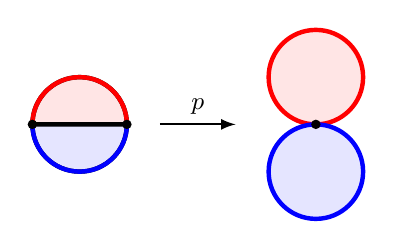
\begin{tikzpicture}[scale=0.6]
\filldraw[red!10, draw=black, line width=1.6pt] (-1.0,0) -- (1.0,0) arc(0:180:1.0) -- cycle;
\filldraw[blue!10, draw=black, line width=1.6pt] (-1.0,0) -- (1.0,0) arc(0:-180:1.0) -- cycle;
\draw[red, line width=1.6pt] (1.0,0) arc(0:180:1.0);
\draw[blue, line width=1.6pt] (1.0,0) arc(0:-180:1.0);
\fill (-1, 0) circle (0.1);
\fill (1, 0) circle (0.1);

\draw[thick, ->, >=latex] (1.7,0) -- node[anchor=south] {\small $p$} (3.3,0);
\filldraw[red!10, draw=red, line width=1.6pt] (5, 1) circle (1);
\filldraw[blue!10, draw=blue, line width=1.6pt] (5, -1) circle (1);
\fill (5, 0) circle (0.1);
\end{tikzpicture}
\end{equation*} 
\end{nn}


\begin{nn}
For any $n\geq 1$, a map $f\colon (X, A, x_{0}) \to (Y, B, y_{0})$ induces a map 
\[
f_{\ast}\colon \pi_{n}(X, A, x_{0}) \to \pi_{n}(Y, B, y_{0})
\] 
given by $f_{\ast}([\omega]) = [f\circ\omega]$. For $n\geq 2$, the map $f_{\ast}$
is a homomorphism of groups. In this way we obtain functors
\begin{align*}
\pi_{1}\colon \Top^{2}_{\ast} \to &\ \  \Set_{\ast} \\
\pi_{2}\colon \Top^{2}_{\ast} \to &\ \  \Gr  \\
\pi_{n}\colon \Top^{2}_{\ast} \to &\ \  \Ab  \\
\end{align*}
\vskip -8mm
for $n\geq 3$, where $\Top^{2}_{\ast}$ is the category of pointed pairs $(X, A, x_{0})$
as objects and maps of such pairs as morphisms.
\vskip -8mm
\end{nn}

\begin{proposition}
If $f, g\colon (X, A, x_{0}) \to (Y, B, y_{0})$ are maps such that $f\simeq g$ (as maps 
of pointed pairs) then $f_{\ast} = g_{\ast}\colon \pi_{n}(X, A, x_{0})\to \pi_{n}(Y, B, y_{0})$
for all $n\geq 1$. 
\end{proposition}


\begin{nn}{\bf Long exact sequence of a pair.}
Consider a pointed pair $(X, A, x_{0})$. The inclusion $i\colon (A, x_{0}) \hra (X, x_{0})$
induces homomorphisms  $i_{\ast}\colon \pi_{n}(A, x_{0}) \to \pi_{n}(X, x_{0})$ for $n\geq 0$. 
Also, the map of pointed pairs $j\colon (X, x_{0}, x_{0}) \to (X, A, x_{0})$ 
induces homomorphisms
\[
j_{\ast}\colon \pi_{n}(X, x_{0}) = \pi_{n}(X, x_{0}, x_{0}) \to \pi_{n}(X, A, x_{0})
\]
for $n\geq 1$. We also have homomorphisms 
\[
\partial \colon \pi_{n}(X, A, x_{0}) \to \pi_{n-1}(A, x_{0})
\]
defined as follows. For $\omega\colon (I^{n}, \pint^{n}, J^{n-1})\to (X, A, x_{0})$, let 
$\omega’\colon (I^{n-1}, \pint^{n-1}) \to (A, x_{0})$ be the restriction of
$\omega$ to $I^{n-1}\times \{0\}$. Then $\partial([\omega]) = [\omega’]$.

\begin{equation*}
\begin{tikzpicture}[
    scale = 1.8,
    d0/.style = {line width = 1.6pt},
    d1/.style= {postaction={decorate}, line width = 1.6pt, decoration={markings, mark=at position 0.55 with {\arrow{stealth}}}},
    d2/.style = {postaction={decorate}, line width = 1.6pt, decoration={markings, mark=at position 0.54 with {\arrow[rotate=9]{stealth}}}},
]

\draw[d0, fill = mygray1] (0,0) rectangle node {$I^{n}$} (1,1);
\draw[d0, red]  (0,0)  --  node[below] {$I^{n-1}\times \{0\}$} (1, 0); 
\fill[] (0, 0) circle (0.04);
\fill[] (1, 0) circle (0.04);

\filldraw[mygray1, draw=black, line width=0.7pt] (2, -0.2) rectangle (4, 1.2);
\filldraw[red!20, draw=red, line width=0.7pt] (2.2, 0.0) rectangle (3.5, 0.7);
\node[anchor=north east, red] at (3.5, 0.7)   {$A$};
\fill[] (2.4, 0.2) circle  (0.04) node[above] {$x_{0}$};

\node[anchor=north east] at (4, 1.2)   {$X$};
\draw[thick, ->, >=latex] (1.25, 0.5) -- node[anchor=south] {\small $\omega$} (1.7, 0.5);

\draw[red,thick, ->, >=latex] (1.05, -0.22) to[out=-15, in=-135] 
node[pos= 0.36, anchor=south] {\small $\omega’$} (2.2, 0.0);
\end{tikzpicture}
\end{equation*}
\end{nn}

\begin{theorem}
\label{HOMOT GPS EXACT SEQ PAIR THM}
For any pointed pair $(X, A, x_{0})$ the following sequence is exact: 
\begin{multline*}
{\dots}\lra \pi_{n+1}(X, A, x_{0}) \overset{\partial}{\lra} 
\pi_{n}(A, x_{0}) \overset{i_{\ast}}{\lra}
\pi_{n}(X, x_{0}) \overset{j_{\ast}}{\lra}
\pi_{n}(X, A, x_{0}) \overset{\partial}{\lra} {\dots} \\
{\dots} \overset{j_{\ast}}{\lra} \pi_{1}(X, A, x_{0}) \overset{\partial}{\lra} 
\pi_{0}(A, x_{0}) \overset{i_{\ast}}{\lra} 
\pi_{0}(X, x_{0}) 
\end{multline*}
\end{theorem}

\begin{proof}
Exercise.
\end{proof}

\begin{note}
The end of the exact sequence in Theorem \ref{HOMOT GPS EXACT SEQ PAIR THM} consists of maps 
of pointed sets. Given such maps 
\[
(S_{2}, s_{2}) \overset{f}{\lra} (S_{1}, s_{1}) \overset{g}{\lra} (S_{0}, s_{0})
\]
exactness at $S_{1}$ means that $f(S_{2}) = g^{-1}(s_{0})$.
\end{note}







